\section{Hardware \dcsecondauthorshort}
%\subsection{Fahrzeug}
Das genutzte Modellfahrzeug wurde von Mitarbeitern der Professur für diese Arbeit und folgende Projekte aufgebaut. Es handelt sich um ein autoähnliches Allrad-Chassis im Maßstab 1:18, an welchem für die Navigation notwendige Umbauten ausgeführt wurden (s. Abb. \ref{fig:tucar_foto}).
\begin{figure}[htbp] % [htb]
	\centering
	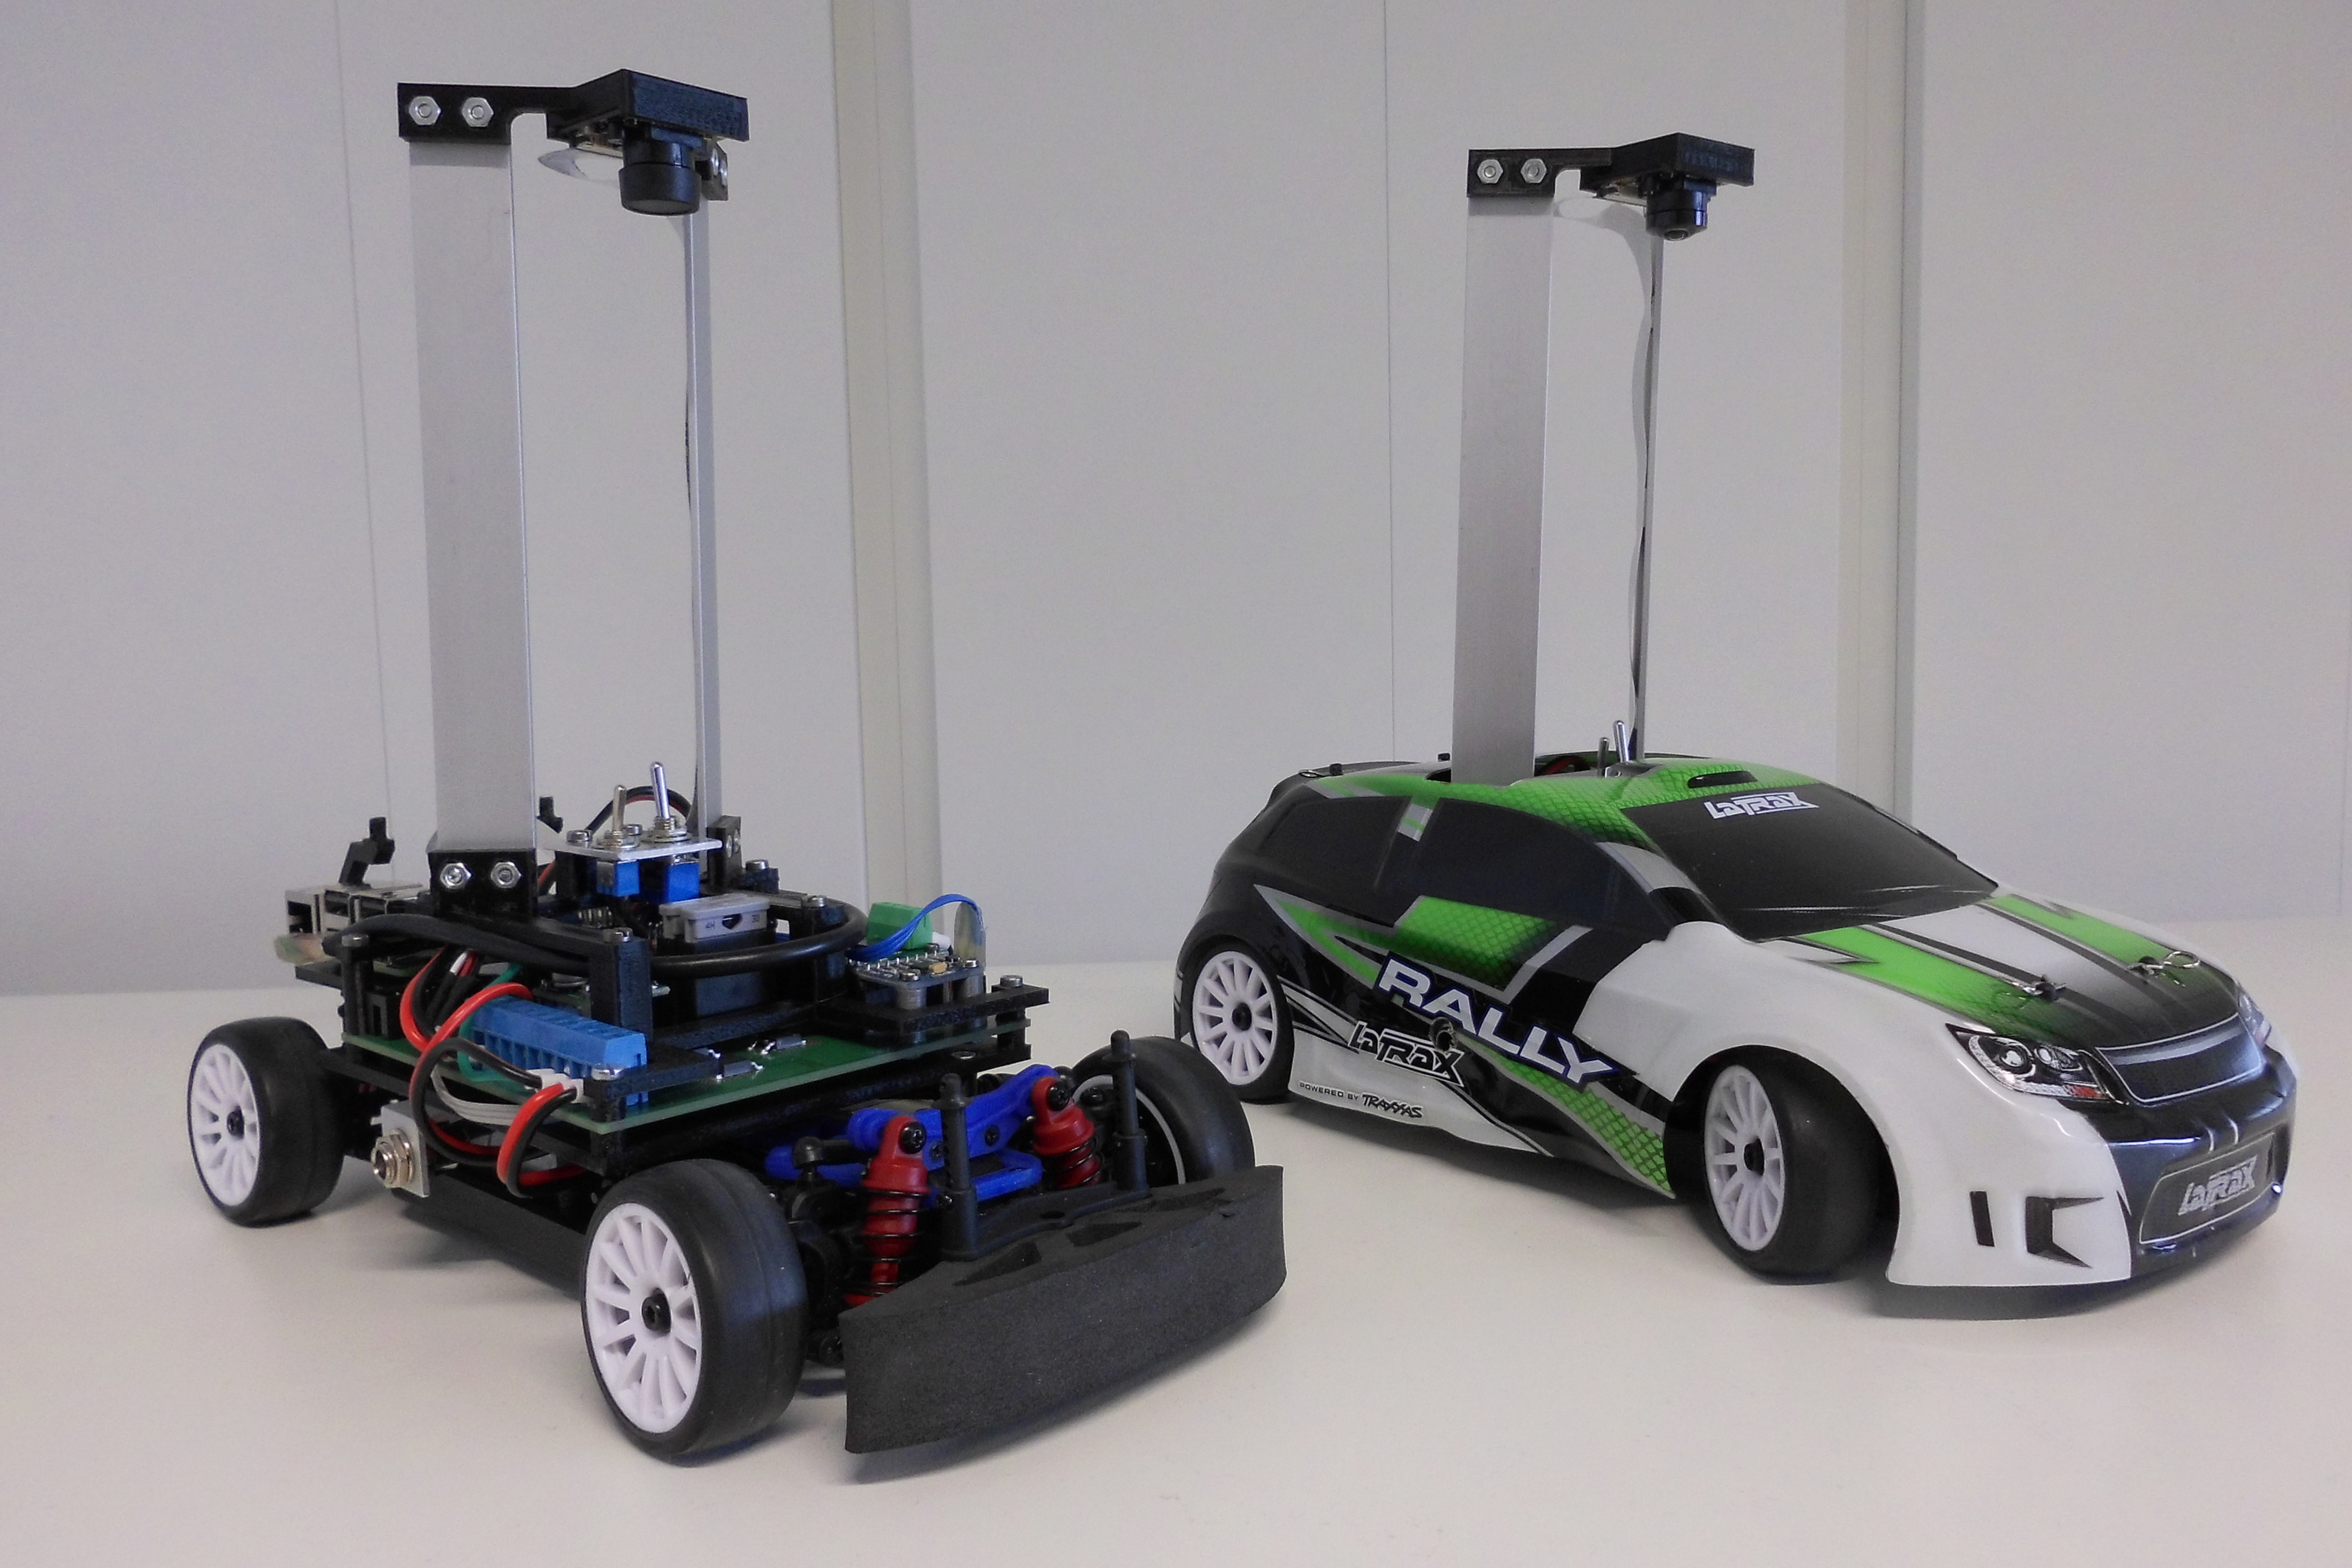
\includegraphics[width=0.8\textwidth]{tucar_foto.jpg}
	\caption{Modellfahrzeug \glqq TUCar \grqq}
	\label{fig:tucar_foto}
\end{figure}
\paragraph{Motor}
Der originale Elektromotor wurde gegen ein Modell mit Encoder ersetzt, da Odometrieinformationen für die implementierte Regelung unerlässlich sind. Zusätzlich ist dem Motor ein Getriebe nachgeschaltet, welches ein Fahren mit langsameren Geschwindigkeiten ermöglicht. Tests mit wenig optimierten Algorithmen werden somit signifikant erleichtert.
\paragraph{\gls{acr:imu}}
Um eine genauere Bestimmung der Pose zu ermöglichen, ist eine \gls{acr:imu} zur Ermittlung der axialen sowie radialen Geschwindigkeiten und Beschleunigungen am Fahrzeugs angebracht. Auch die durch numerische Integration erhaltene Orientierung kann direkt von diesem Modul abgefragt werden. 
\paragraph{Kamera}
Neben der Odometrie und \gls{acr:imu} stellt eine in Vogelperspektive angebrachte Kamera mit Fisheye-Objektiv die einzige Sensorik des Fahrzeugs dar.
\paragraph{Rechentechnik}
Zur Ansteuerung der Kamera und zum Entgegennehmen der Fahrbefehle ist ein Raspberry-PI Einplatinenrechner montiert, dessen WLAN-Schnittstelle zum Informationsaustausch mit dem Fahrzeug dient.
